Pela visão de auxiliar pesquisadores em suas integrações de modelos de ML com simuladores de redes ópticas elásticas, as análises aqui feitas devem buscar o aumento de produtividade do pesquisador. Para isto, as tecnologias de ML analisadas serão avaliadas de forma qualitativa, sendo esta avaliação guiada pelas seguintes questões:

\begin{itemize}
  \item Há algum custo para usar a tecnologia?
  \item O código da tecnologia é aberto?
  \item A tecnologia é ativamente mantida por \textit{maintainers} e/ou pela comunidade?
  \item O uso da tecnologia é amplamente documentado?
  \item A instalação e uso da tecnologia é simples?
  \item A tecnologia permite a execução de modelos pré-treinados?
  \item A tecnologia permite a execução de modelos pré-treinados com outras tecnologias?
\end{itemize}

Nesta análise, apenas tecnologias com licenças de código aberto serão consideradas de modo que os pesquisadores tenham livre acesso às recomendações e sejam capazes de manipulá-las em seus projetos, caso seja necessário. Dentre essas, apenas tecnologias disponíveis para uso em programas Java ou Python serão consideradas.

A linguagem Java é amplamente utilizada para a implementação de simuladores de redes ópticas elásticas, como em \cite{costa2016ons}, \cite{ceons2015} e \cite{net2plan}, por isto, a integração de modelos de ML de forma embutida no simulador permite uma integração performática ao excluir-se a necessidade de comunicação com outros serviços ou processos para executar os modelos.

\begin{figure}[h]
  \centering
  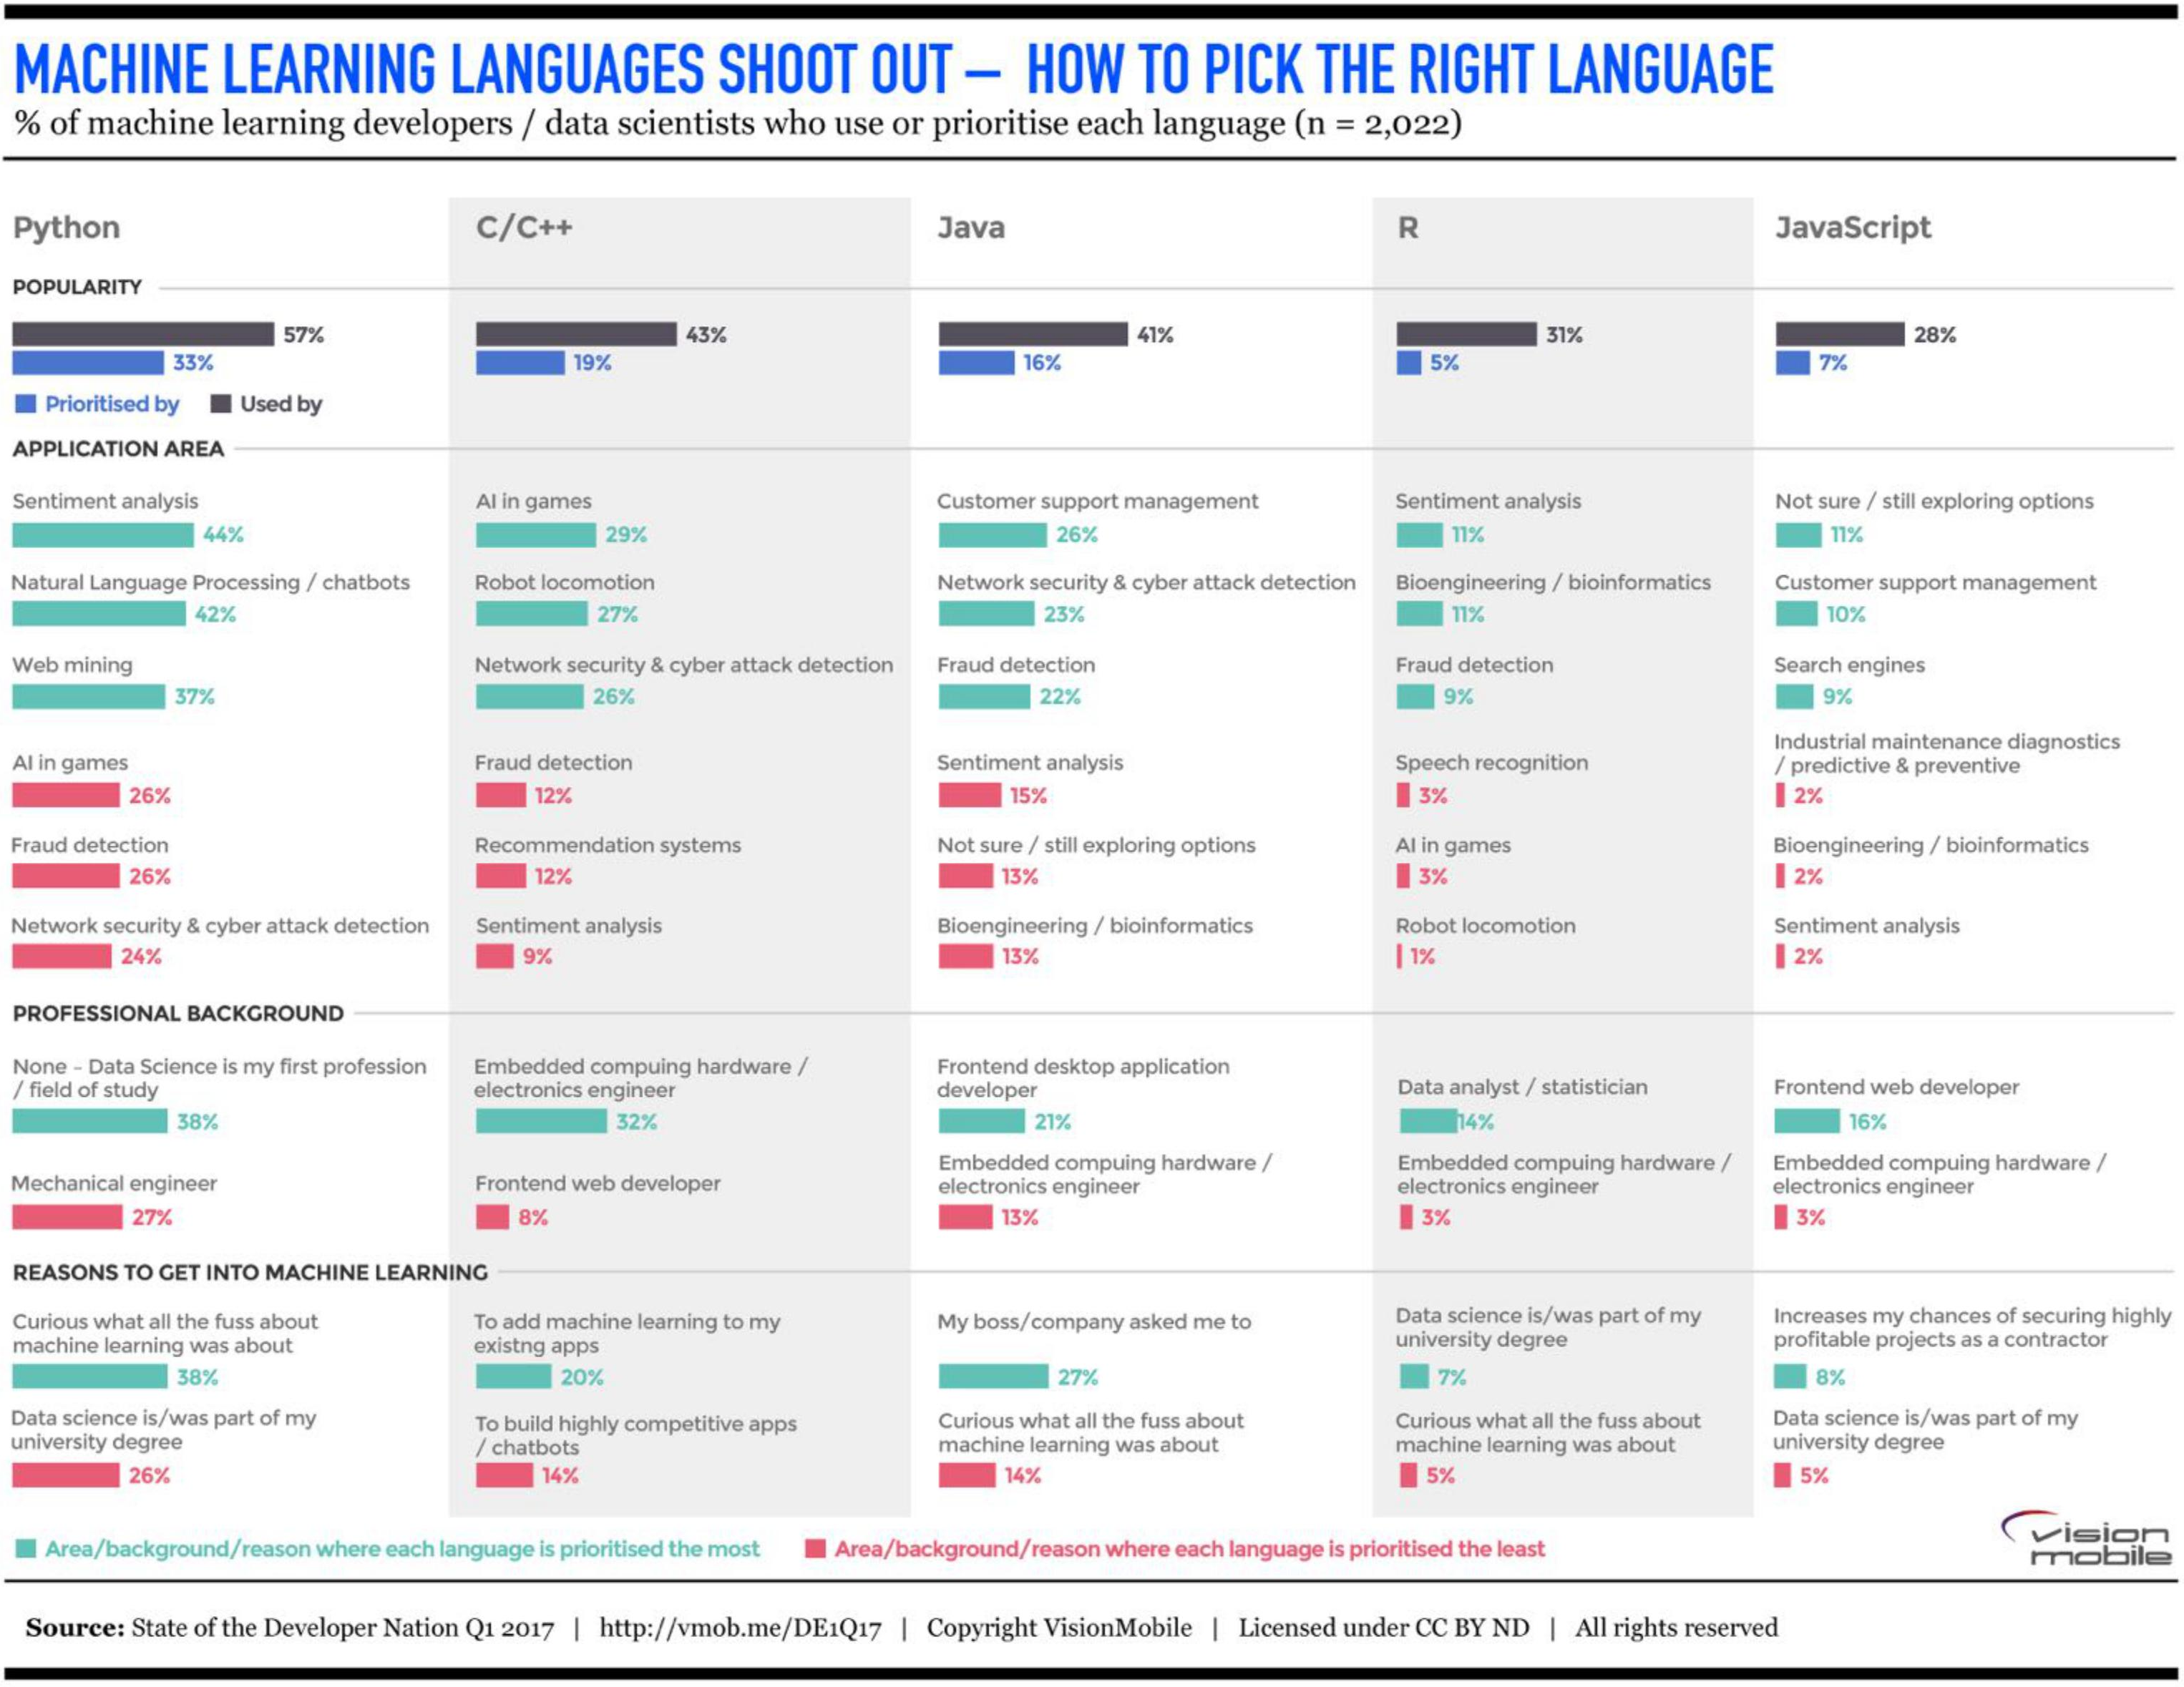
\includegraphics[width=1\textwidth]{img/languages-ml.png}
  \caption{Porcentagem de cientistas de dados e desenvolvedores de inteligência artificial que usam ou priorizam cada linguagem \cite{developer_nation_q1_2017}}
  \label{fig:languagesml}
\end{figure}

A linguagem Python é a mais usada e priorizada para desenvolvimento em ML entre trabalhadores da área, como evidenciado na figura \ref{fig:languagesml}. Assim, uma integração de simuladores com um processo ou serviço independente escrito em Python, responsável por executar os modelos, pode ser mais fácil de ser desenvolvida e mantida por um pesquisador de ML na área de EONs, apesar do custo de tempo da execução graças ao tempo necessário para comunicação entre os processos ou serviços.

As tecnologias também devem ser fáceis de serem instaladas, configuradas e manipuladas de acordo com as necessidades de cada pesquisador. Para isto, é fundamental que suas APIs sejam bem documentadas e que a instalação exija o mínimo de modificações de configurações da máquina, externas ao simulador.

Por fim, o uso de ML se expande por diversos problemas relacionados à EONs, de modo que estes problemas podem beneficiar-se de diferentes tipos de aplicações de ML, de acordo com suas características. Assim, é ideal que a tecnologia de ML escolhida para integração com o ML tenha suporte a diferentes tipos de modelos.

\section{OpenCV}

OpenCV (Open Source Computer Vision Library) é uma biblioteca de código aberto voltada para visão computacional e aprendizagem de máquina, construída para fornecer uma infraestrutura comum para aplicações de visão computacional e acelerar o uso de percepção de máquina em produtos comerciais \cite{ml_site_opencv}.

Apesar do foco principal de OpenCV ser visão computacional, a biblioteca possui um módulo de redes neurais profundas e interfaces para as linguagens Python e Java. Adicionalmente, também é possível realizar a importação de modelos serializados em diversos formatos, como Darknet \cite{ml_site_darknet}, Torch7 \cite{ml_site_torch}, ONNX \cite{ml_site_onnx} e TensorFlow \cite{ml_site_tensorflow}.

A API da biblioteca é extensamente documentada, porém com poucos tutoriais sobre o uso do módulo de DNNs. Entretanto, no quesito facilidade de instalação e configuração os resultados foram variados:

Em Python, para a execução de modelos com apenas o uso da CPU a instalação se resume a instalar o pacote \texttt{opencv-python-headless}, a versão sem dependências de bibliotecas de interfaces de usuário gráficas, e está pronto para uso. Porém, se há interesse em utilizar a GPU na execução dos modelos, o processo de instalação se torna bastante complexo, sendo necessário compilar manualmente a biblioteca considerando diversas configurações do ambiente da máquina, de modo que a criação de uma solução generalizada se torne inviável.

Em Java, o processo de instalação é complexo independente do uso ou não de GPU, sendo necessário o mesmo processo de compilação manual do projeto considerando configurações da máquina, não havendo nenhuma integração com gerenciadores de pacotes populares como \textit{Maven} ou \textit{Gradle}.

Assim, pelas dificuldades presentes na instalação, o único uso de OpenCV considerado é o de Python com as execuções sendo realizadas apenas pela CPU da máquina, sem uso de GPU.

\section{PyTorch}

PyTorch é uma biblioteca de ML de código aberto que provê uma plataforma de pesquisas em aprendizagem profunda, oferecendo máxima flexibilidade e velocidade \cite{pytorch_what_is}, sendo considerada a biblioteca de aprendizagem profunda que mais cresce no mundo \cite{course_fast_ai}. Na análise da biblioteca, não foram encontrados métodos nativos de conversão de modelos para serem inferidos com o uso de PyTorch e por este motivo o seu uso foi descartado.

\section{Scikit Learn}

\textit{Scitkit-learn} é uma biblioteca de código-aberto desenvolvida em Python que integra diversos algoritmos de ML para problemas supervisionados e não-supervisionados de média escala com ênfase em trazer ML para não-especialistas \cite{scikit-learn}. É uma biblioteca extremamente popular, principalmente entre iniciantes na área de ML, com desenvolvimento ativo na comunidade.

A biblioteca, com suporte apenas para Python, possui extensa documentação de modo a melhor auxiliar iniciantes. Pelo seu foco em simplicidade, a biblioteca não possui suporte para uso de GPU em treinos ou execuções de modelos. Para importação e exportação de modelos, a biblioteca conta apenas com serialização nativa de Python por meio da biblioteca \textit{pickle}, não sendo possível importar modelos de outros formatos.

Apesar da facilidade de se desenvolver modelos de ML com \textit{Scikit Learn}, o uso da biblioteca foi descartado pela falta de suporte ao uso de GPU e de importação de modelos pré-treinados salvos em formatos diversos.

\section{TensorFlow}

\section{TensorFlow Lite}

TensorFlow Lite \cite{ml_site_tensorflow_lite} é uma \textit{framework} de aprendizagem profunda para execução de modelos em dispositivos. Se trata da versão da popular \textit{framework} TensorFlow que é projetada para execuções em dispositivos com menor poder computacional.

A importação de gráficos é limitada apenas a arquivos do tipo TFLite, porém existem ferramentas para realizar a conversão de formatos comuns em Tensorflow, como Keras e SavedModel. Atualmente, a biblioteca não fornece suporte a execução com uso de GPUs NVIDIA \cite{ml_site_tensorflow_lite_gpus}.

Tendo os fatores acima em consideração, a instalação e uso da biblioteca são simples e amplamente documentados para programas Python. Para a instalação, é necessário instalar a versão do pacote específica para a versão do interpretador Python instalado na máquina, sendo possível configurar uma detecção automática. A biblioteca não possui versões para uso em programas Java que não sejam voltados para Android.

Apesar da limitação de importação de modelos e a impossibilidade de uso em programas Java, TensorFlow Lite será avaliado de forma quantitativa pelo seu foco específico de execução rápida de modelos em dispositivos de borda.

\section{ONNX Runtime}

A ONNX Runtime \cite{ml_site_onnx_runtime} se trata de um acelerador de treinamento e execução de modelos de ML salvos em formatos ONNX \cite{ml_site_onnx}. O formato ONNX é um formato aberto construído para ser uma representação comum de modelos de ML, possuindo amplo suporte em s bibliotecas de ML.

A ONNX Runtime é desenvolvida com foco em suporte cross-plataforma, fornecendo uma API comum para diversas linguagens como C, C++, Java e Python. Seu desenvolvimento é apoiado por diversas empresas como Microsoft, Facebook, IBM, Intel, NVIDIA, entre outras.

Graças ao foco de implementações cross-plataforma, a instalação das bibliotecas para Java e Python são simples e exigem pouca ou nenhuma configuração. Em ambos os casos, é necessário apenas instalar o respectivo pacote caso a intenção seja usar apenas a CPU para inferências. Se houver interesse em usar uma GPU NVIDIA, é necessário instalar a versão da \textit{runtime} compatível com a versão de CUDA instalada.

A documentação da biblioteca possui poucos guias ou tutoriais mas conta com diversos exemplos de código em Python para operações comuns e um exemplo de código em Java, além da completa referência dos pacotes de ambas versões da biblioteca.

Apesar da documentação limitada, a ONNX Runtime será considerada na avaliação de desempenho pela alta portabilidade da biblioteca, sendo ideal para atender aos diferentes casos de uso de pesquisas de ML em EONs.

\section{DeepLearning4j}

Eclipse DeepLearning4j \cite{ml_site_deeplearning4j} é uma biblioteca de código-aberto para aprendizagem de máquina distribuída, disponível para Java e Scala. Seu desenvolvimento está ativo e é conduzido pela empresa Konduit.

A biblioteca possui ampla documentação da API e diversos tutoriais que explicam os diferentes usos da biblioteca. É possível importar modelos no formato ONNX, HDF5 e TensorFlow, além de seu próprio formato.

A instalação da biblioteca é extremamente simples para uso de CPU e se dá por meio do gerenciador de pacotes Maven, sendo necessário apenas adicionar apenas algumas linhas na configuração do projeto para que seja possível executar o DeepLearning4j. Para uso de GPU, apenas máquinas com placas de vídeo NVIDIA e com CUDA configurado são suportadas. Neste caso, o processo de instalação é quase o mesmo, tendo como diferença o identificador da biblioteca que depende da versão da GPU instalada na máquina.

A biblioteca DeepLearning4j será avaliada em um programa Java com uso de ambas CPU e GPU.

\section{MXNet}

A biblioteca MXNet \cite{ml_site_mxnet} é uma \textit{framework} de código-aberto para aprendizagem profunda que permite a definição, o treinamento e a execução de redes neurais profundas em diversas plataformas, estando atualmente em desenvolvimento, em processo de incubação pela Apache Incubator. Se trata de uma biblioteca bastante versátil, com suporte à diversas linguagens, incluindo Java e Python, e importação de modelos em formato ONNX para execução.

Entretanto, o suporte para Java é limitado primeiramente no quesito disponibilidade de bibliotecas. Alguns arquivos binários presentes no pacote possuem licenças incompatíveis com a licença Apache 2, resultado na retirada dos pacotes de Java do repositório Maven. Assim, para utilizar uma versão atualizada da biblioteca é necessário compilar o código-fonte. Além disso, a documentação para Java também é quase vazia, tendo apenas dois tutoriais simples e a publicação da referência da API. Pela dificuldade de instalação e a falta de tutoriais e suporte da comunidade, o uso de MXNet para Java foi descartado.

A versão em Python da biblioteca MXNet é bastante completa, contando com diversos tutoriais para diferentes casos de uso, além de prover uma fácil instalação por meio do gerenciador de pacotes \textit{pip}. Entretanto, em testes iniciais para avaliar a viabilidade de uso da biblioteca, foi descoberto que a bibliteca dispara erros ao tentar executar o modelo usado pelo autor \cite{eon_ml_classifier_2020} para a comparação de desempenho entre as bibliotecas, logo o uso de MXNet para Python também foi descartado.

\section{Keras}

\section{Outras tecnologias}

